\documentclass[9pt,conference]{IEEEtran}
\IEEEoverridecommandlockouts
% The preceding line is only needed to identify funding in the first footnote. If that is unneeded, please comment it out.
\usepackage{cite}
\usepackage{amsmath,amssymb,amsfonts}
%\usepackage{algorithmic}
\usepackage{graphicx}
\usepackage{textcomp}
\usepackage{xcolor}
\usepackage{todonotes}
\usepackage[ruled,vlined]{algorithm2e}
\usepackage{threeparttable}



\newcommand*\circled[1]{\tikz[baseline=(char.base)]{
		\node[shape=circle,fill,inner sep=0.5pt] (char) {\textcolor{white}{#1}};}}
		
\def\BibTeX{{\rm B\kern-.05em{\sc i\kern-.025em b}\kern-.08em
    T\kern-.1667em\lower.7ex\hbox{E}\kern-.125emX}}
\begin{document}

%\title{Accelerating FM-index for Next-Generation Sequencing Data Processing in 3D-Stacked Memory}
\title{Accelerating FM-index Search for Next Generation Sequencing Analysis with 3D-stacked Memory}
\maketitle

\begin{abstract}
In bioinformatics, the Ferragina-Manzini Index (FM-Index) is an important algorithm across a wide range of genomic data analysis applications such as sequence alignment, data compression, and genome annotation. The massive genomic data produced by various genome sequencing technologies presents a significant challenge for genome analysis based on FM-index. 
Recent effort has accelerated FM-index by using SIMD, FPGA, and ASIC. However, its massive random memory access and exploration of genomic data contribute to huge data movement between processing units and memory in traditional von Neumann architectures.
Inherent parallelism in FM-index is extremely challenging for conventional systems as well due to their severe memory bandwidth limit.

In this paper we argue that the processing-in-memory (PIM) concept could be a viable solution to address these challenges.
We propose an application-driven near-data processing accelerator for FM-index using 3D-Stacked memory which facilitates stacking logic and memory dies. 
In order to achieve memory-capacity proportional performance by taking advantage of this new technology, we propose (1) a new architecture that fully take advantage of the available memory bandwidth, (2) a lightweight message passing mechanism between memory vaults, and (3) a hardware prefetcher specialized for memory access patterns. 
Our evaluation shows that the proposed architecture can achieve 20$\times$/1820$\times$ speedup when compared with the best available ASIC solution and 32-thread CPU baseline, respectively.
\end{abstract}

\section{Introduction}
Precision medicine has become a promising and an efficient approach to clinical diagnosis that allows patients to be treated with the personalized medicine based on a genetic understanding of their disease. For instance, people with melanoma, leukemias, and different kinds of cancers, e.g., breast, lung, colon, and rectal, usually have their tumours to be tested for certain genetic changes when they are  diagnosed~\cite{shendure2008next,chang2016smem,cong2017aim}. 
It is predicted that by 2025, 1 billion people will have their own genome records, which will generate up to 40 exabytes genomic data per year~\cite{stephens2015big}. 
This increasing huge data in turn has led to a upsurge of genetic analysis tools~\cite{}.

The first and critical processing step is alignment, which performed per-read group and consists of mapping each individual read pair to the reference genome. Basically, all alignment algorithms generally follow a \textit{seed-and-extend} model, where \textit{seed} represents a sequence index-search to collect all candidates of exact matches, and \textit{extend} is an inexact match to extend the candidates with a scoring method. 
Depending on different generations of sequencing~\cite{}, the time cost of seed and extend varies sharply. 
The reason is that the de facto standard for \textit{extend} is Smith-Waterman dynamic programming algorithm with time complexity as \textit{\textit{O}($N^2$)}, where \textit{N} is the length of sequence reads. 
Commonly, the length of sequence reads of NGS is as short as $50 - 200$ base-pairs (A, C, G, T), which is much shorter than that of the first or the third generation of sequencing. 
Unfortunately, Darwin-like coprocessors are not designed to process such short reads since its thousand times speedup depends on the parallelism exposed by aligning long reads (e.g., $>$1K base-pair). Darwin coprocessors work well on alignment algorithms for long sequence reads only and when \textit{extend} dominates mapping time.
However, when processing NGS reads, \textit{extend} is not the performance bottleneck. 
The execution time of the most widely used reads alignment tool BWA~\cite{li2013aligning} is dominated 29\% to 70\% by the prior procedure \textit{FM-index search} of \textit{extend} to find exact matched seeds. However, FM-index has not been well studied because of its two challenges: 

\textcolor{blue}{
First, massive random memory access leads to huge data movement between processing units and memory on traditional von Neumann architecture~\cite{}, which results in resulting in bottlenecks of both performance and energy~\cite{}. Various compute-centric hardware approaches, such as multi-core~\cite{}, GPU~\cite{}, and FPGA~\cite{} have been explored to accelerate DNA seeding. However, innovations that only focus on the computation have limited space for improvement, since DNA seeding is memory bound~\cite{}. 
}

\textcolor{blue}{
Second, \textit{system performance is limited by the main memory capacity and bandwidth per server.} Due to the pin count limitation per chip, For instance, Kocberber et al.~\cite{Kocberber:2013bb} observed that using more than four index traversal units. Wang et al.~\cite{yuanrong} observed that using more than 48 PEs will not provide additional speedup due to off-chip bandwidth limitations.
}

In this paper, we show that processing-in-memory (PIM) can be a key enabler to accelerate genomic data processing with memory-capacity-proportional performance under the current pin count limitation. 
To investigate the potential benefits of PIM, we first delve into a critical algorithm, FM-index, to understand what underlying functions and characteristics contribute the most to data movement. From our observation, FM-index is with simple functions and primitives (which we refer to as small computation) that are responsible for a significant fraction of the total data movement. Therefore, PIM architectures are promising for design FM-index accelerators to overcome the bandwidth bottleneck. Our design is driven by application characteristics and budget of device. First, due to the strict area budget of PEs of FM-index, the compute logic is required to be fairly simple yet efficient; Second, inherent massive parallelism in FM-index drives an efficient mechanism for communication between PEs resided on a the logic layer of PIM. 

The main contributions of this paper are as follows:

\begin{itemize}

    \item We observe that data movement between the main memory and computation units is a major contribution to the total system cost for FM-index. The most of it is generated by simple operations such as basic arithmetic operations, and bitwise operations, which can be parallelly implemented in simple hardware logic.
    
    \item We propose a new design of an application-driven accelerator, called GeneF, for FM-index algorithm that can effectively utilize processing-in-memory (PIM). We propose an efficient mechanism for communication between different PEs, which can hide long remote access latencies via the use of non-blocking message passing. We introduce a specialized prefetcher that decouple data access logic from PEs, which can fully pipeline compute and data access.
    
    \item Our evaluations show that GeneF outperforms the best available ASIC solution by 20$\times$. Compared to the state-of-the-art software solution BWA-MEM on conventional systems, we get 1820$\times$ performance speedup and 7032$\times$ energy efficiency gain.
    
\end{itemize}

\section{Background and Motivation}
\subsection{Algorithm Description}
FM-index~\cite{bwt} is the widely used kernels in many alignment tools~\cite{ahmed2016comparison}, which follows the seed-and-extend model. The seeding stage needs to \textbf{exactly} align seeds of the reads back to the reference genome without any gap. An FM-index is created by first taking the Burrows-Wheeler transform (BWT) of the input text in the following steps. For example, \circled{1} the genome string T = "abracadabra\$", \circled{2} and here it is represented by the matrix M where each row is a rotation of the text, and the rows have been sorted lexicographically. \circled{3} The BWT of the genome string T = "abracadabra\$" is "ard\$rcaaaabb", which is the last column labeled \textbf{L} of matrix M. The data structure has two features, the first xxx. The second is is the i character occurrence of a character c in the last column has the same rank as the ith occurrence of c in the first column. Thus, searching the query seed is done by a last-to-first mapping with the fomula, which can be defined as LF(i) = C[c] + Occ(c, i). The C[L[i]] represents the number of symbols in BWT that are lexicographically smaller than character a. Occ(L[i], i) is the number of occurrences of a in the BWT string of the reference genome based on current position i, C[L[i]].

\begin{algorithm}[!htbp]
\LinesNumbered
\caption{FM-index based Seeding Algorithm}\label{algo:fm}
\small
\KwIn{Query sequence $SD[d]$, Reference genome $R[len]$}
\KwOut{Matching locations}
%Preprocess: Derive $B_R[len]$, $S_R[len]$, $C_R[4]$, and $O_R[len+1][4]$;\\
\While{$sp <= ep$ and $i >= 2$} {
    $c \leftarrow P[i-1]$;\\
    \lIf{$x = EoF$} {\textbf{break}}
    $sp = C[c] + Occ[c, sp-1]+1$;\\
    $ep = C[c] + Occ[c, ep]$;\\
    $i \leftarrow i - 1$;\\
}

\lIf{$ep < sp$}{\Return $Not \ found$}
\lElse {\Return $ep - sp + 1$}
\end{algorithm}

\subsection{FM-index Search on Conventional Systems}
FM-index search is a challenging task for conventional system. Our profiling results in Figure~\ref{fig:data-fm} quantitatively shows the bottleneck. As Figure~\ref{fig:data-fm} shows, the DRAM access accounts for 60\% in the CPI stack analysis; The number of Load/Store instructions takes 43.4\% among total number of instructions in Figure~\ref{fig:data-fm}; The energy breakdown shows that 49.4\% of total energy consumption is consumed by the DRAM. We find that the main reason of huge data movement and the suitability for PIM execution. For each base \textit{m}, new values of \textit{sp} and \textit{ep} are computed by accessing two locations of the \textit{Occ} structure. These locations depend on m and the current values of \textit{sp} and \textit{ep}. There is no defined pattern between successive values of \textit{sp} and \textit{ep}. While \textit{Occ} is a huge data structure. Accessing the elements stored in the BWT index requires pointer-chasing and is also referred to as FM-index-search (FIS). FIS is intrinsically a sequential operation because of the data dependency to the next address, and also often accesses random addresses. Thus, architectural advances in modern processors (e.g., multiple cache hierarchies, MLP, and prefetching) provide limited performance improvement for this phase. In addition, while the computation for FIS is relatively simple as shown in~\cite{yuanrong}, the main-memory latency is critical to the overall performance, which cannot be handled by the current memory hierarchies. Previous work~\cite{yuanrong} shows that for FM-index search, only a few types of operations are dominative, e.g., memory copy operations, bitwise operations, and simple arithmetic operations like integer addition/subtraction and integer shifting. Many other operations are needless, such as floating-point operations, multiplication/division, vector and other complicated operations. In short, FIS is characterized by a large number of data movements generated by simple operations. This lead to the key question in this paper: \textit{how can we provide large amounts memory bandwidth to such simple operations?}

\begin{figure}[!htbp]
\centering
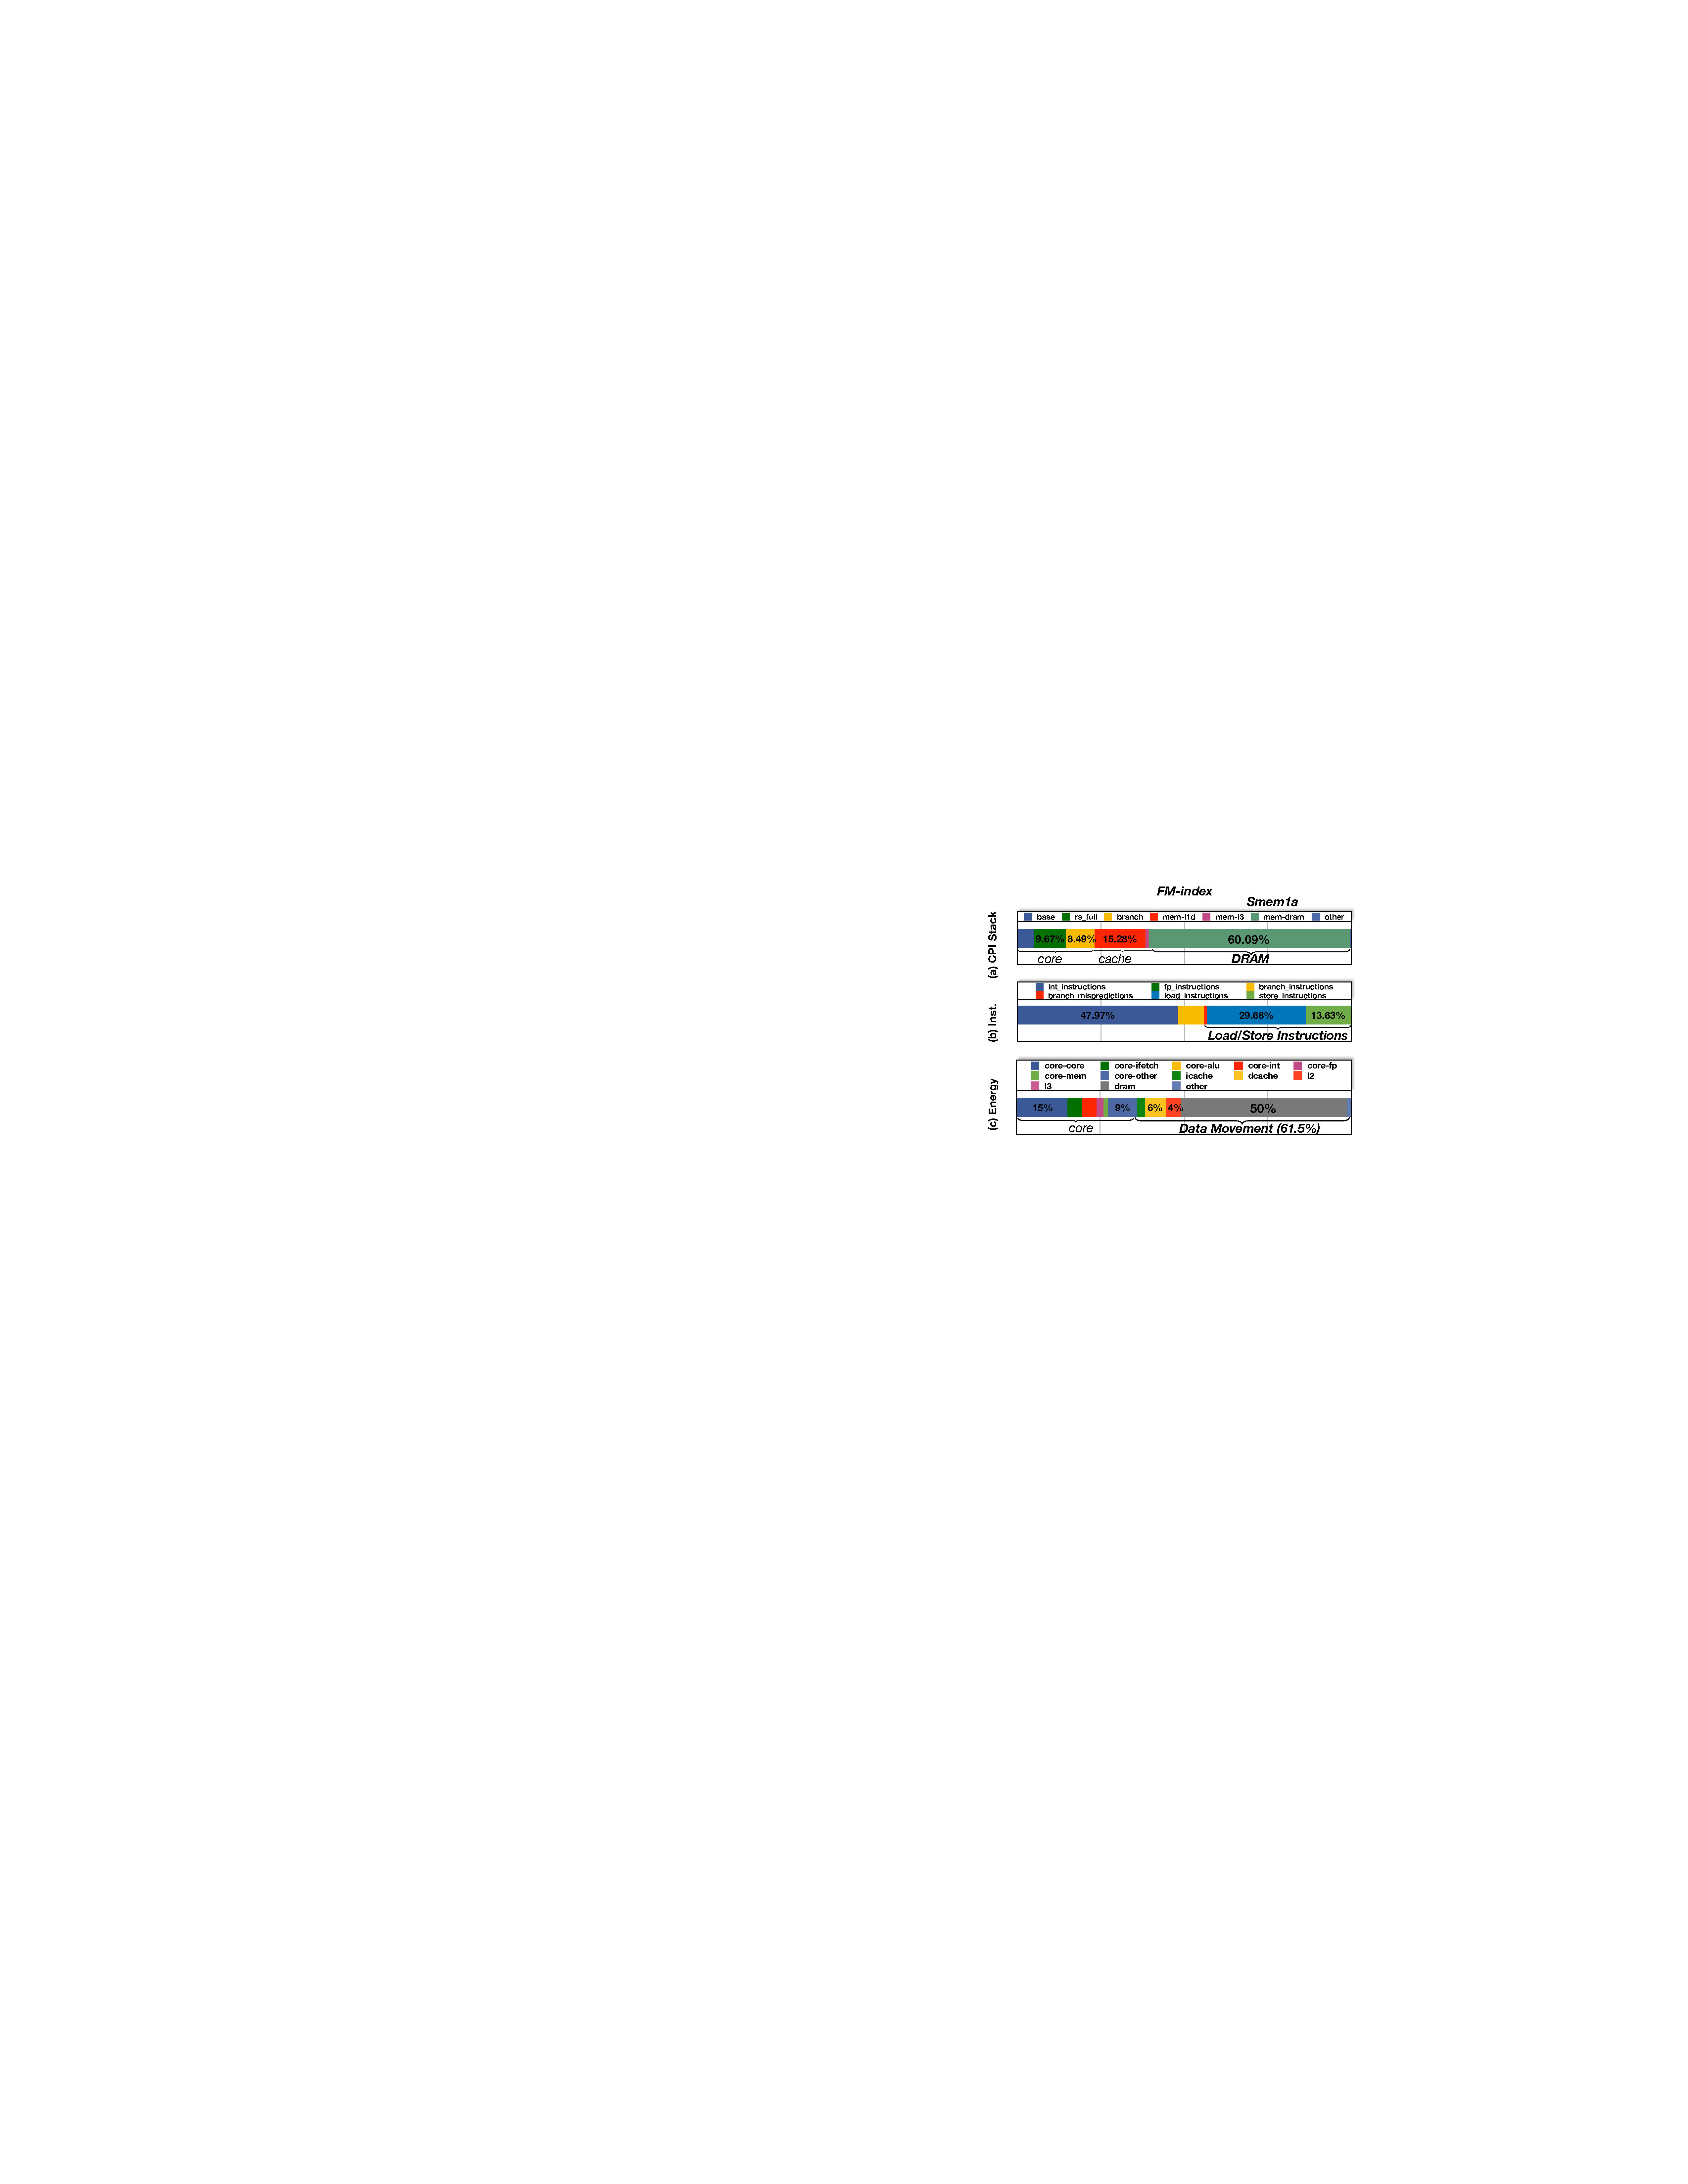
\includegraphics[scale=0.4]{Conference-LaTeX-template_10-17-19/fig/data-fm.pdf}
\caption{Profiling the FM-index kernel in BWA-MEM with Sniper and configuration in Table II: (a) CPI stack; (b) Instruction statistics; (c) Energy breakdown.}
\label{fig:data-fm}
\end{figure}

\subsection{Processing-in-Memory}
\textit{Processing-in-memory} (PIM) has becoming a promising solution due to the emergence of 3D-stacked DRAM architecture, which stack multiple DRAM layers using vertical \textit{through-silicon vias} (TSVs) to provide much greater bandwidth between layers. 3D-stacked DRAM architectures (e.g., HBM~\cite{3Dstacking}, HMC~\cite{3Dstacking}) involve a base \textit{logic layer} within the stack. Considering a system composed of 16 8GB HMCs as an example, conventional processors are still limited to 320 GB/s of memory bandwidth assuming that the CPU chip has the same number of off-chip links as that of an HMC. In contrast, PIM exposes 8 TB/s (= 16 Cubes $\times$ 512 GB/s) of aggregate internal bandwidth to the in-memory computation units. This internal bandwidth, which can be expanded with memory capacity, is very important for big data applications. By moving computation inside memory, PIM can satisfy the high memory bandwidth requirement of FIS. The access location in the BWT table jumps irregularly with large strides. there seems to be little locality between consecutive access locations. The irregular memory access is the main reason for the high. PIM will reduce huge data movement and short access latency. Furthermore, the behaviors of individual seeding tasks, i.e., the elemental task for parallel computing, are independent, PIM will provide high parallelism. However, moving compute logic inside memory brings two critical questions: (1) How to design an architecture that fully utilize the internal memory bandwidth? (2) how to communicate between different partitions to be performed in parallel?

\section{GeneF Architecture}
\label{sec:arch}

\begin{figure*}[t]
\centering
%\vspace{-3pt}
%\includegraphics[width=\linewidth]{fig/hpca20-v4.pdf}
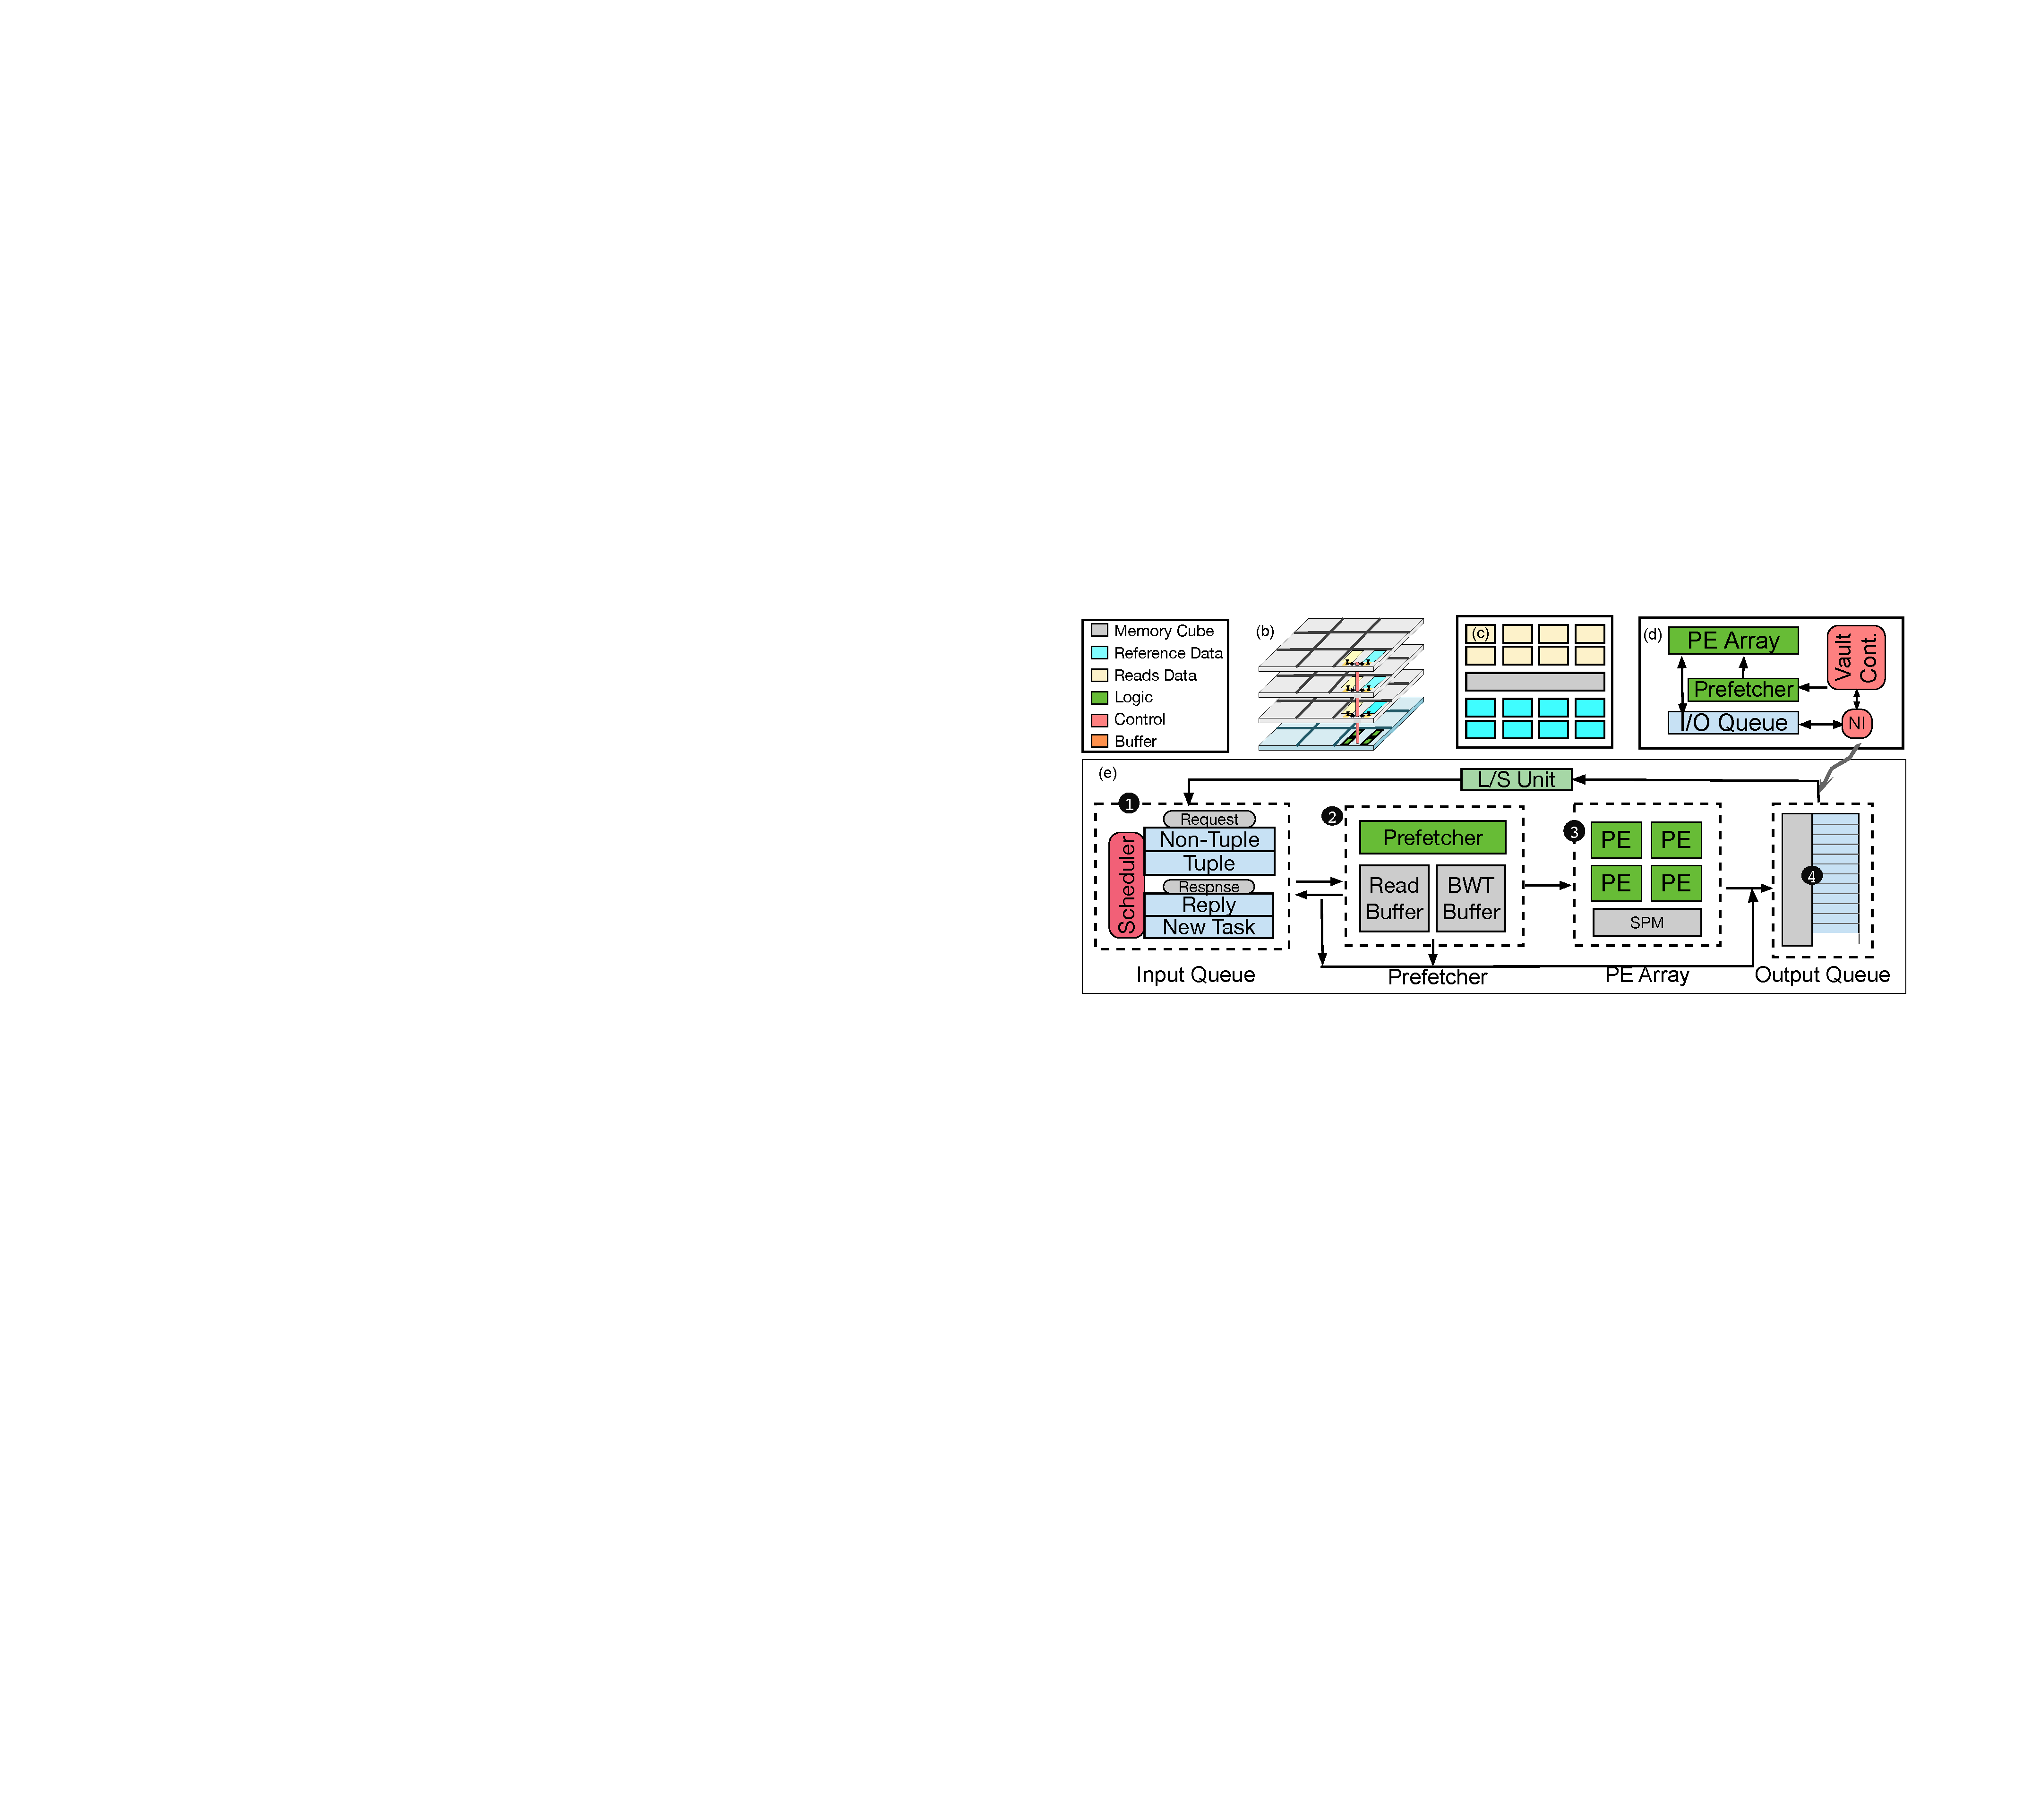
\includegraphics[scale=0.5]{Conference-LaTeX-template_10-17-19/fig/arch.pdf}
\caption{Architecure overview of GeneF accelerator (a) Network of Cubes, (b) Overview of a cube, (c) Data Mapping (d) Vault overview, (e) Compute Logic}
\label{fig:arch_design}
\end{figure*}

%This section elaborates the design of GeneF. We start with GeneF overview in Section~\ref{sec:arch:overview}.
%The Data Mapping Mechanism is further elaborated on in Section~\ref{sec:arch:data}. We introduce a Lightweight Message Passing Mechanism in Section~\ref{sec:arch:message}. Then we take a look at the Prefetch Mechanism to enable each GeneF core to exploit the high available memory bandwidth in Section~\ref{sec:arch:prefetch}. Finally, we explore the number of PE configurations under each vault in Section~\ref{sec:arch:pe_number}.

\subsection{Overview}
\label{sec:arch:overview}
Figure~\ref{fig:arch_design} shows a conceptual diagram of the proposed architecture. GeneF is composed of 16 HMC cubes and provides 128GB of memory capacity as shown in Figure~\ref{fig:arch_design}(a). Figure~\ref{fig:arch_design}(b) depicts an HMC cube structure consisting of eight 8Gb DRAM memory layers and one logical layer. Each HMC is vertically divided into 32 regions (called Vault). These Vaults are connected by an on-chip network. We divide 32 vaults of each HMC into 2 groups as shown in Figure~\ref{fig:arch_design}(c), so that each group of vaults can store one reference genome (blue square), and the other half part can store DNA sequences (yellow square) (Section~\ref{sec:arch:data}). 
Figure~\ref{fig:arch_design}(d) depict the logic layer and design details can be seen in Figure~\ref{fig:arch_design}(e). We put the customized RISC-V based processing elements (PEs) on the logic die. These PEs can be replaced. We choose light message passing to communicate between PEs under different vaults (Section~\ref{sec:arch:message}). To keep PEs simple, PEs in GeneF is only responsible for the calculation. We decouple the data-access function from the computation logic (Section~\ref{sec:arch:prefetch}).  Prefetcher~\circled{2} mainly prefetches reference genome data and the DNA sequences. With the prefetcher, required data can be ready for PE before local calculation is performed. The Input Queue~\circled{1} and Output Queue~\circled{4} are the interfaces that the vault logic layer interacts with the on-chip network. The Output Queue as the egress will send out the processing requests to the remote vault, while the Input Queue serves as the ingress to receive the request and results from the remote. Thanks to the independent processing between reads, these HMC cubes can store the reference genome and read separately, which makes the computation inside HMC independently. This execution mode makes the overall internal bandwidth of the system up to 8TB/s. 


%\subsection{Data Mapping}
%\label{sec:arch:data}
%We first depict the organization of data layout. Taking human genome as an example, the reference genome is about 3 GB size. The BWT-based gene comparison application requires frequent random access to the BWT sequence of the reference sequence. In order to eliminate the frequent access overhead of the external storage device, reference sequence needs to be stored in the memory. However, the capacity of an HMC cube is only 8GB. The storage space of each vault of the HMC is only 256MB. It is impossible for PEs under one vault cannot performan alignment by simply accessing the above vault. 

%Due to the existence of built-in DRAM controllers, HMCs use a packet-based protocol for communication through the inter-lintra-HMC network instead of low-level DRAM commands as in DDRx protocols, we divide the genome data into small blocks, which are stored in different memory areas (vaults), and realize data communication between vaults through the on-chip network.

%The straightforward way is to divide the reference sequence is divided into 32 parts and stored in 32 vaults. Each vault uses its own memory controller that provide packet-based remote access mechanisms to communicate with other vaults. This method will also make the average distance of remote access larger and affect performance. In fact, half capacity of HMC cube, which is 4GB, can fully accommodate the reference genome. In our design, we divide all the 32 vaults into 2 groups. Each vault of each group is connected with 2D mesh network. The reference sequence data is divided into 16 parts and distributed over the vault of each group as shown in Figure~\ref{fig:arch_design}(c). In this way, the computing unit within each vault can access not only the local storage tier, but also the storage tier reference sequence data of other vaults through a very fast on-chip network.

\subsection{Lightweight Message Passing Mechanism}
\label{sec:arch:message}
Unlike host processors that have access to the entire address space of the HMCs, each GeneF core is restricted to access its own local DRAM partition only. However, access to the reference sequence is random throughout the sequence. As shown in Figure~\ref{fig:non-block}(a), to process data from a remote vault, PE under local vault needs to sends the data request to the remote vault. The remote vault accesses the data and access the corresponding data, and sends it back to the local vault, which requests the data. Finally, local PE performs subsequent operations. However, two outstanding problems must be kept in mind: (1) the PE of the local vault is blocked since it is waiting for data, so the utilization rate is reduced with the affect of the overall performance, (2) the amount of network communication data is huge, a factor which brings a large amount to the on-chip network pressure. Taking FM-index as an example, for the \textit{Occ4} function process, in each LF mapping iterative calculation, two pieces of BWT rank data corresponding to \textit{sp} and \textit{ep} are required, and each rank data amount is 64 Byte, so each iteration needs to pass 2x64=128 Byte data. Coupled with the data requested, this bulk data transfer will put a lot of pressure on the on-chip network since the on-chip network bandwidth is only 16B/cycle~\cite{gao2015practical}.

To solve the challenge, we moves computation to the target PEs that contains the data to be processed, instead of allowing remote memory accesses. We propose a lightweight message passing mechanism, which is employed for communication between different DRAM partitions.

\textbf{Definition.}~The lightweight message definition is shown in Figure~\ref{fig:message}, where the meaning of each field is explained as follows:

\begin{figure}[htbp]
    \centering
    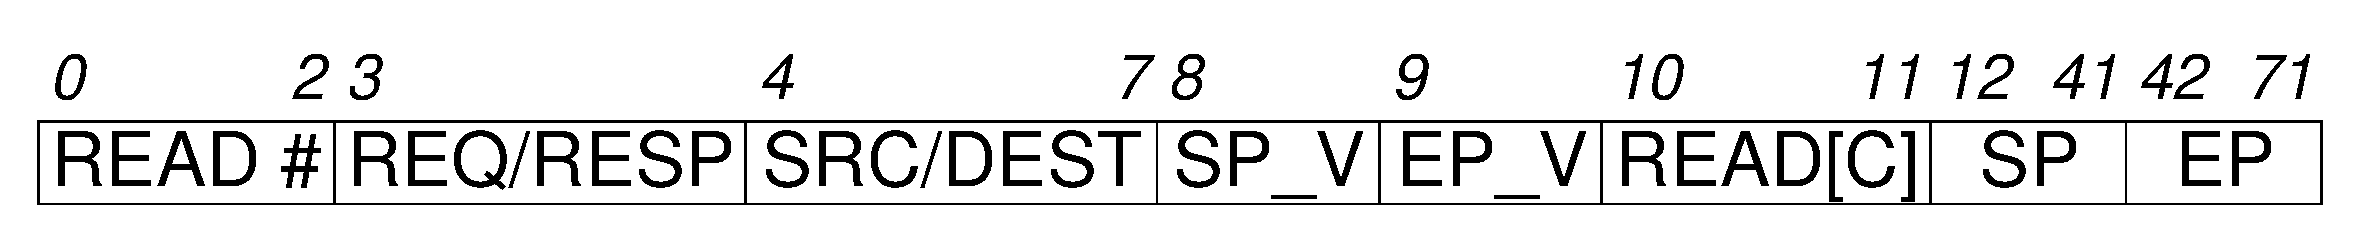
\includegraphics[width=\linewidth]{fig/Bits.pdf}
    \caption{Lightweight Message Passing}
    \label{fig:message}
    %\vspace{-0.5cm}
\end{figure}


\begin{itemize}
    \item \textit{READ\#:}~Request or respond to the corresponding read number. We have 4 to 8 read spaces reserved for the read slot in the Input Queue, so the ID only needs 3-bit to represent.
    
    \item \textit{RES/RESP:}~Request or response ID, this field only needs one bit to mark.
    
    \item \textit{SRC/DEST:}~Source vault and destination vault ID. Since each group of vaults is numbered from 0 to 15, this field requires only 4 bits.
    
    \item \textit{SP\_V/EP\_V:}~SP/EP valid flag bit. These two flags respectively mark whether the SP and EP fields in this message are valid, 1 represents valid, and 0 represents invalid.
    
    \item \textit{READ[C]:}~This field stores 2 bits of the target base of the current iteration.
    
    \item \textit{SP/EP:}~The index (and the updated index) storage area. The request message needs to carry the (sp,ep) index value, and the reply message also needs to return the updated (sp,ep) index. Both sp and ep in the original algorithm require 64-bit storage. According to the reference address range and the range of vault access, only 30 digits can meet the needs.
\end{itemize}


\begin{figure}[htbp]
    \centering
    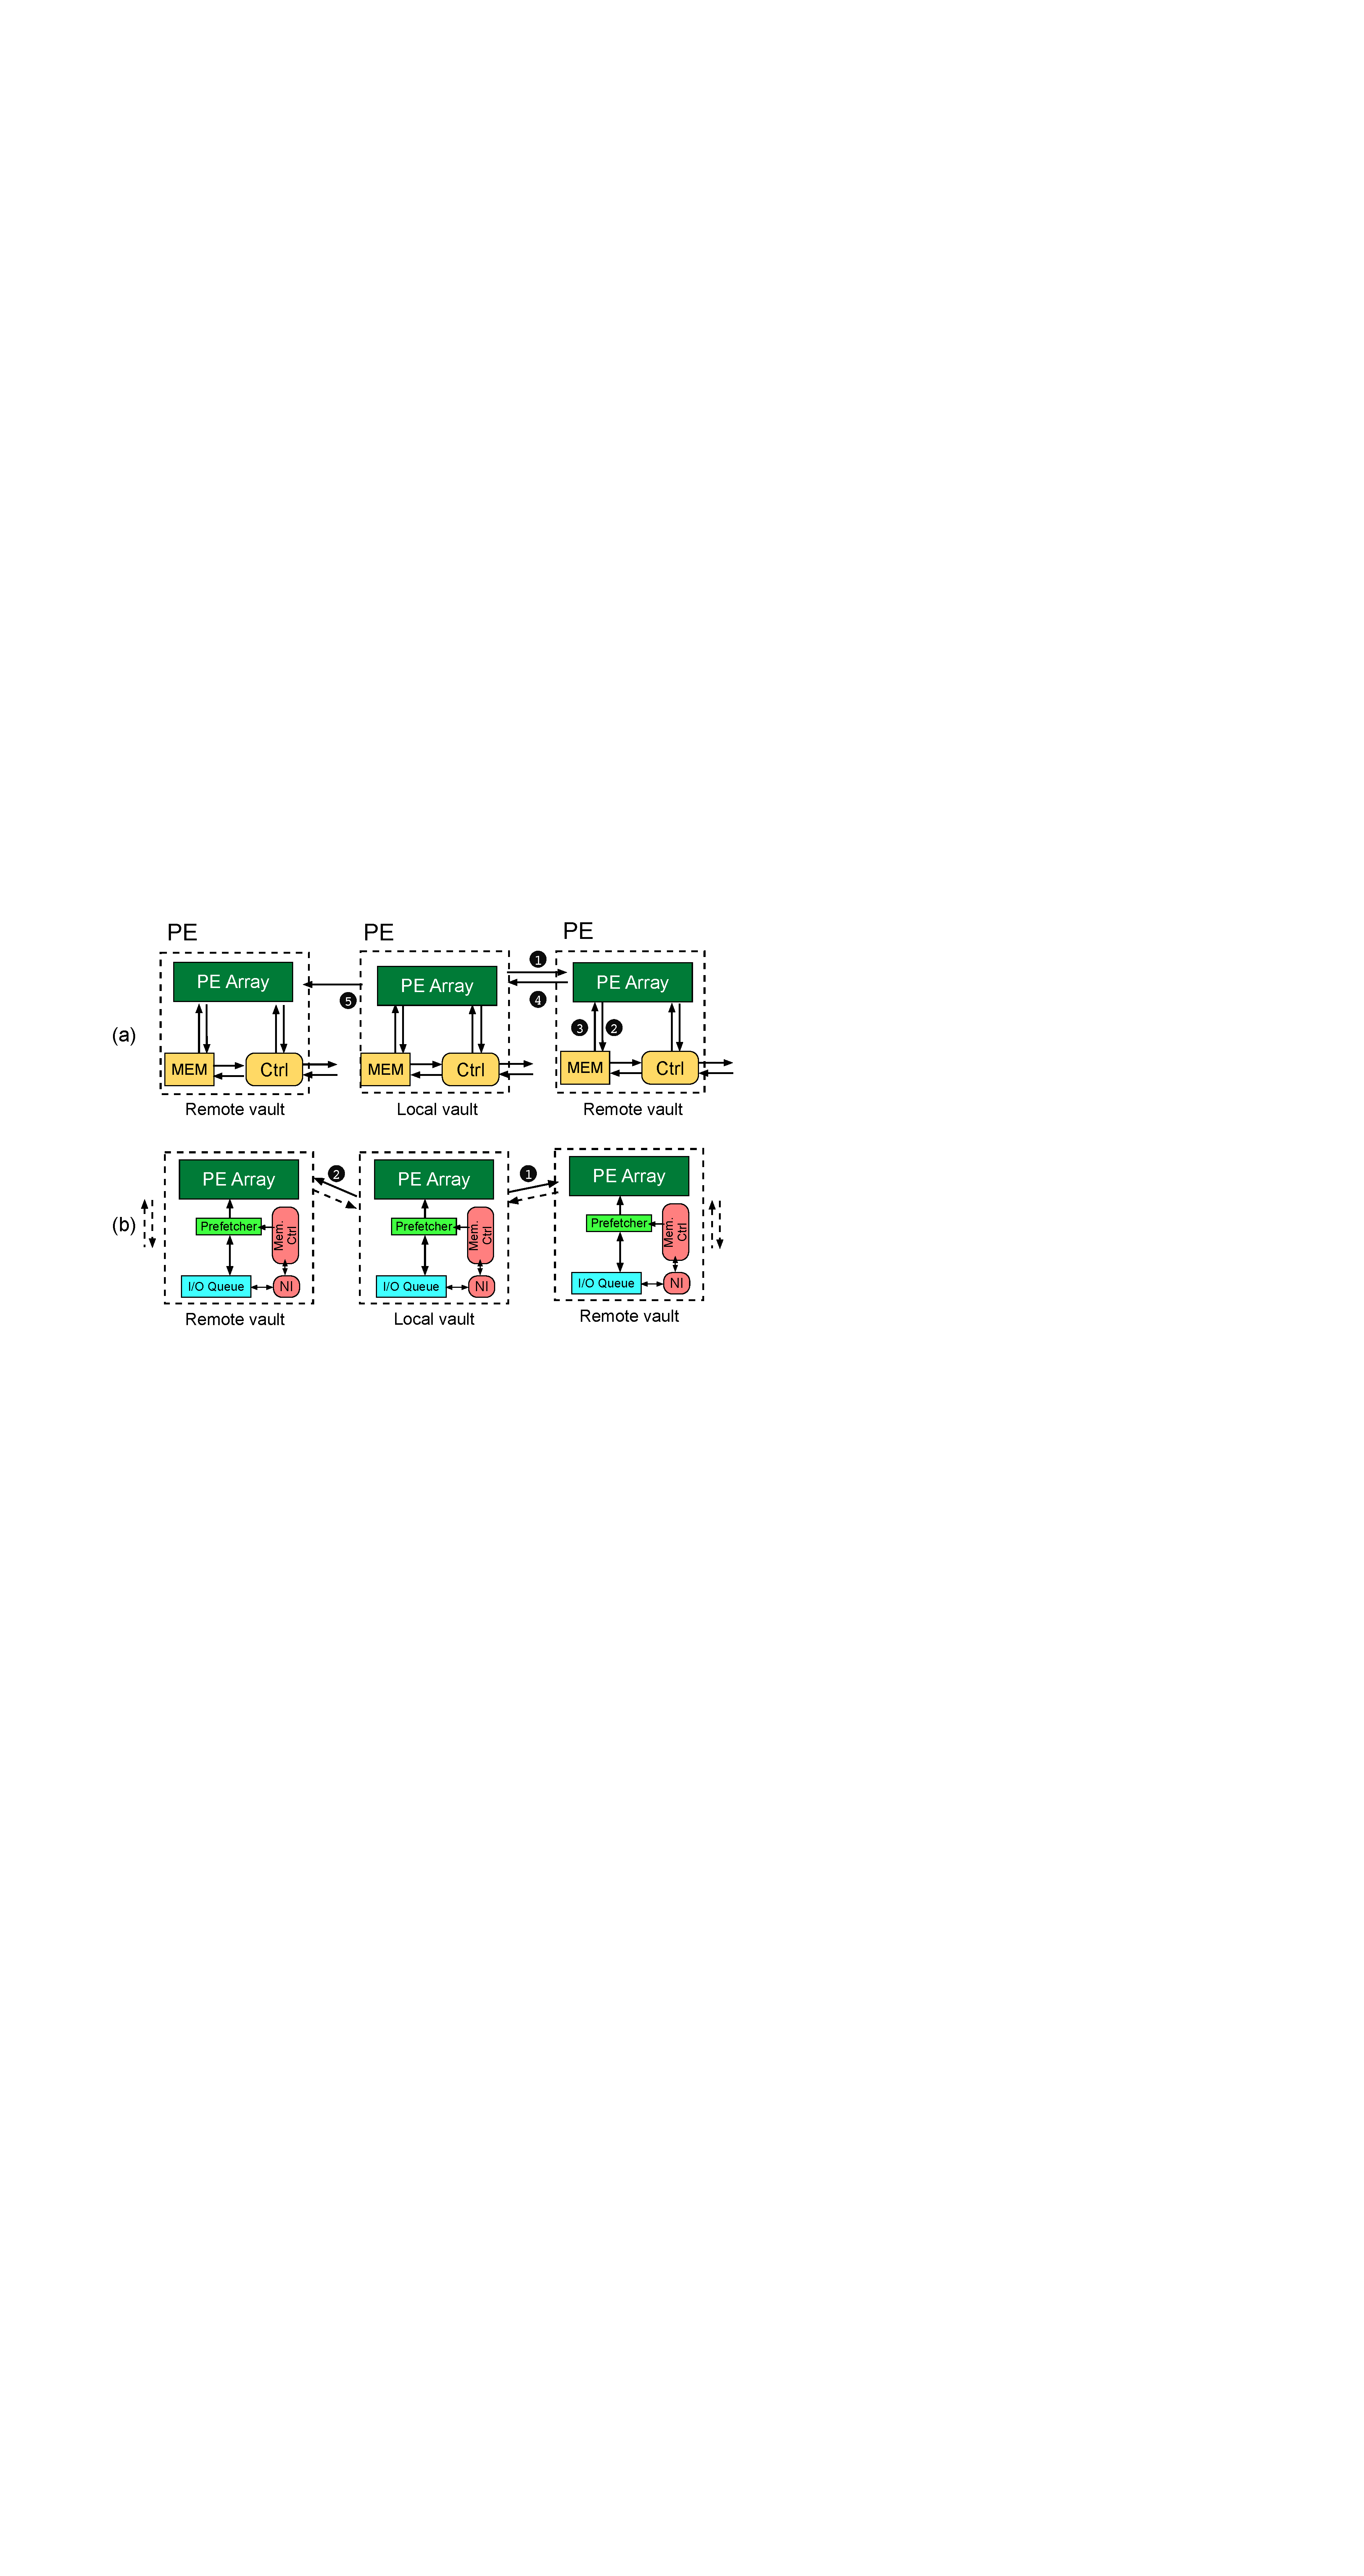
\includegraphics[scale=0.3]{fig/message.pdf}
    \caption{Non-Blocking Remote Function Call}
    \label{fig:non-block}
\end{figure}

When the local vault is performing LF mapping, if the required BWT data is not on the local storage vault but on the remote vault, the local vault sends the data address and other parameters to the remote vault. After the vault receive the message, the remote vault directly performs data access and subsequent calculation operations by itself before finally returning the calculation result (the updated index value) to the source vault, which avoids the overhead of the move of huge BWT data. Based on the above design method, the lightweight message defined in this paper only accounts for 72 bits (9 bytes). Compared with the transmission of 128 bytes of BWT data, this lightweight message is combined with the way that move the computation to the target core that contains the data to be processed. As shown in Figure~\ref{fig:non-block}(a), the source vault needs to wait for the destination vault to return data after sending a data request to the destination vault or processing the request. Or the result is processed, and the source vault can only in idle state during this period. Although this communication method is the most intuitive, the problem of resource idleness and waste is serious, which causes the throughput of the processing unit to decrease.

\textbf{Non-Blocking Remote Function Call.}~We then propose Non-blocking Remote Function Calls mechanism shown in Figure~\ref{fig:non-block}(b). In this mechanism, after the source vault sends a message to the destination vault to process the request, it allocates a corresponding slot in the scheduler in the Input Queue. We add a message queue to each vault that stores messages for non-blocking remote function calls. Functions in this queue are executed once the queue is full. This means that other components do not need to wait for the return result, and can fetch the processing request sent by other vaults to continue the computation and memory access or process the return value. The exact sequence of performing a non-blocking remote function call is as follows:

\begin{itemize}
    \item The source vault sends a request message to the destination vault, and then the source vault continues other processing.
    
    \item The destination vault receives the processing request.
    
    \item The destination vault prefetches the BWT data according to the location pointer in the message.
    
    \item The destination vault assigns a task to the PE for an iterative calculation to obtain a new index value.
    
    \item The destination vault returns the updated index as the response source vault.
    
    \item The source vault receives a response from this task and waits for subsequent task scheduling.
\end{itemize}

%This mechanism greatly helps to optimize the performance of remote function calls in two ways. 
First, this mechinism enables the data communication between the vault, the task processing on the vault is also well flowed, a factor which eliminates the overhead of the source vault idle. Second, remote function call execution is not preempted by other remote function calls.

\subsection{Prefetching}
\label{sec:arch:prefetch}
In accelerator~\cite{yuanrong}, each PE can process an LF mapping iteration completely. The PE first requests memory access according to the iterative processing flow. Each PE contains an address translation unit (AU) and a memory access unit (MU), they take the BWT data back from the memory, and then perform the vector calculation operation through the calculation unit (CU), which means that the PE needs to wait for the data to return during the memory access phase. However, massive parallelism can masks the memory access latency of a single PE. 

For PIM, although putting a core beneath memory exposes unprecedented memory bandwidth to the core, it is far from the best way of utilizing ample memory bandwidth for the
following reasons: (1) PEs need to wait for the data to be returned from remote vault. (2) We can increase the number of PEs to hide the memory access latency. However, the area of logic die limites the number of PEs. Thus, we design a lighter PE which only retains the main computing logic and some accessorial memory units (such as registers and on-chip scratchpad memory). The memory access unit and the address conversion unit are decoupled from the inside of PE to the outside of PE. The memory access unit is placed as part of the prefetcher~\circled{2}, which provides data to the PE continuously through data prefetching. The scheduler~\circled{1} of the input queue performs a simple address translation when requested by the input queue, and then sends the memory address to the prefetcher. The prefetcher performs data access in the vault storage layer according to the corresponding memory address; thus, the data is fetched. It is sent back to the data cache of the PE array~\circled{3} for PE to perform subsequent calculations. For this reason, the memory access and calculation component of each iterative process can be performed in a pipeline, a process that ensures that the PE does not need to wait for data to be fetched. Through the decoupling optimization of computing and memory access with the prefetch mechanisms, each functional component is in the state of pipelined operation, a feature which produces the highest computing efficiency with the least resource consumption.

\begin{figure*}[!t]
\centering
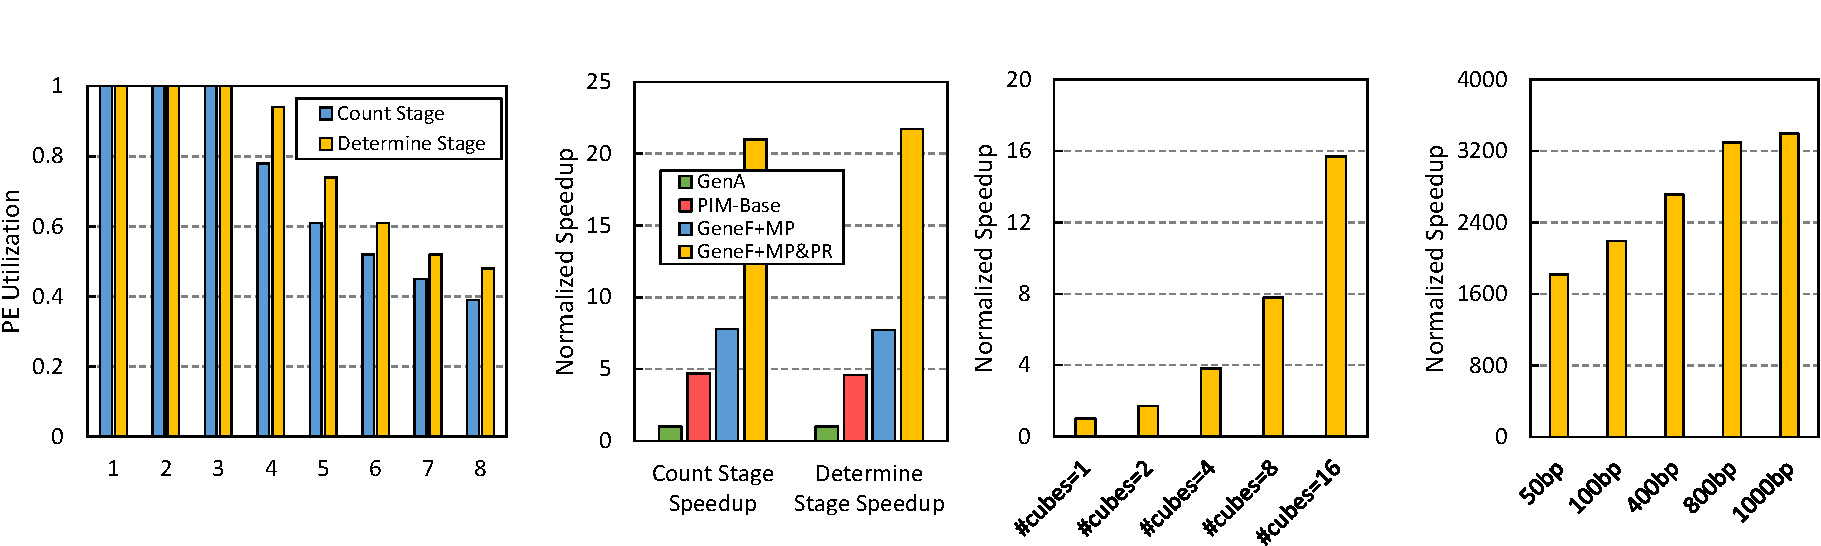
\includegraphics[scale=0.55]{Conference-LaTeX-template_10-17-19/fig/result.pdf}
\caption{Profiling the FM-index kernel in BWA-MEM with Sniper and configuration in Table II: (a) CPI stack; (b) Instruction statistics; (c) Energy breakdown.}
\label{fig:result}
\end{figure*}

\subsection{PE numbers exploration}
\label{sec:arch:pe_number}
After the optimization of computation and memory units using prefetch mechanism, we keep the accelerator simple while maintaing the maximum computational efficiency. However, a single PE design is far from the best way of utilizing the ample memory bandwidth. In order to achieve the effect of parallel processing, which make full use of the ample memory bandwidth, we need to put more PEs on the logic layer of each vault while the speed of data provided by the prefetcher can keep up with the calculation speed of the PEs. The major concern is the balanced number of PEs. 

As shown in Figure~\ref{fig:result} (a), we quantized the number of PEs under each vault and the utilization of PE resource. When the number of PEs on each vault does not exceed three, the calculation rate of the PE array cannot keep up with the rate at which the prefetcher provides data. This leads to the state that although the PE has been operating at 100\% full utilization, it is still insufficient for the consumption of memory bandwidth due to the limitation of parallelism. When the number of PEs is 4, both the \textit{counting stage} and the \textit{determination stage} show that the idle rate of PEs is between 10\% and 20\%, which indicates that the calculation rate of the PE array has exceeded the supply rate of the prefetcher in this case, and the bandwidth has been fully utilized. When the number of PEs exceeds 4, an increasing proportion of PE idle rate will occur, that is, resource waste becomes more and more obvious. Based on this, the PE array of vault is composed of 4 PEs, which can fully utilize the memory bandwidth resources and ensure the effective use of PE resources.
%\vspace{10pt}


\section{Experiment}
\subsection{Experiment Setup}
\subsection{Performance}
Figure~\ref{fig:result} (b) depicts the performance for both our architecture design and baselines. We normalized the performance of Niubility as 1, which took customized computing logic of FM-index and showed 79$\times$ speedup over 32-thread CPU implementation. We based on Niubilitu design with 3D-stacked memory to further improve the memory bandwidth and computing parallelism. Compared to the ASIC implementation, we achieve around 20$\times$ speedup. Compared with the software implementation on the 32-thread CPU platform, the \textit{count} and \textit{determine} stages are 1820$\times$ and 1728$\times$ faster, respectively. The speedup comes from not only the high enough memory bandwidth that HMC provides, but also the corresponding optimization for the new memory structure. We solve the problem of storing reference data by data partitioning and memory area grouping. The non-blocking function-based message passing customization and remote in-place processing mode hide the overhead of remote communication, and achieve the best acceleration effect with the least computational resources through computation-memory decoupling and data prefetching.


\subsection{Message and Prefetch Mechanism Efficiency}
Although the near-memory computing structure can provide more memory bandwidth, which is the basis for massive parallelism. We observed that directly transplant the accelerator into 3D-Stacked memory is far from the ideal performance. As shown in Figure~\ref{fig:result} (b), due to higher memory bandwidth, when we expand the number of PEs from 384~\cite{yuanrong} to 2048, the performance improvement is only 4.7$\times$ and 4.6$\times$ for Count and Determine stages respectively. That is because although we extend the number of PEs to take advantage of memory bandwidth, reference sequence data must be dispersed due to HMC capacity limit. On top of the different vaults of HMC, this brings the latency overhead of remote vault data access, which slows down the overall throughput. We solve the problem using a light message passing mechanism. This mechanism is designed by considering application characteristics as mentioned in Section~\ref{sec:arch}, to hide the overhead of remote communication and eliminate the pressure. As shown in Figure~\ref{fig:result} (b), our message mechanism performs 1.66$\times$ and 1.68$\times$ speedup than PIM-Base. Further, due to the strict limitation of logic layer on power consumption and area, we minimizes the design of PE and decouple computation and data-access part. We improve the utilization of PEs using prefetcher, which makes data be in ready state before computing. Our prefetching mechanism further improves the performance in \textit{count stage} and \textit{determine stage} by 2.69$\times$ and 2.81$\times$, respectively.

\subsection{Scalability}
We study the scalability of GeneF by increasing memory capacity horizontally. Generally, the growing number of PEs indicating a higher parallelism, then the amount of workload assigned to each PE will decrease resulting in a worse locality. This trade-off between parallelism and locality will influence the scalability.

First, we show the scalability of GeneF by increasing the number of cubes in Figure~\ref{fig:result} (c). Figure~\ref{fig:result} (c) shows that GeneF with 2 cubes achieves 1.9$\times$ speedup and with 16 cubes, GeneF achieves 15.7$\times$ speedup on average compared to the default configuration. These results reveal almost linear scalability. This kind of extensibility comes from the comparison of application features and HMC structural features. First, BWT-based gene alignments have natural read-to-read concurrency features. There is no dependency between streaming read inputs. Different reads are processed in parallel; on the other hand, the advantage of BWT-based gene comparison is its smaller memory space, which enables its data volume to be accommodated by a single HMC without data interaction across cubes. Therefore, different HMCs can store reference sequence and read stream data separately and perform irrelevant read processing independently without communication between HMCs, which explains the good scalability of HMC.


\subsection{Sensitivity Study about Read Length}
%Since GeneF is an application-driven accelerator that is specifically designed to accelerate the FM-index algorithm. For applications such as BWA-MEM and Bowtie, all of their core algorithms are based on FM-index, their acceleration for these applications is reflected in the performance improvement of FM-index. As mentioned before, in order to balance the efficiency and accuracy, many applications adopt the seed-extension model, which integrates dynamic programming algorithms (such as Smith-Waterman) on the basis of FM-index exact matching to perform inexact matching expansion of seeds. In order to explore the performance impact of GeneF on these applications, we also need to consider the impact of dynamic programming algorithms. 

We take BWA-MEM as an example, which is the fastest, the most accurate and widely used software based on the seed-and-extended mode. We take the state-of-art optimization Darwin~\cite{turakhia2018darwin} as the baseline of Smith-Waterman algorithm. As shown in Figure~\ref{fig:result} (d), if we only accelerate the dynamic programming part of BWA-MEM, even with the powerful hardware acceleration method in~\cite{turakhia2018darwin}, the overall speedup of BWA-MEM is only 2.2$\times$ higher with 16-thread, due to the FM-index algorithm in BWA-MEM accounts for a large amount of execution time. After using GeneF to optimize FM-index part, combined with the dynamic programming hardware accelerator in~\cite{turakhia2018darwin}, the speedup can be increased by more than 1000 times when read length is 101bp, which is typical with the next generation sequencing technology~\cite{depristo2011framework, fujiki2018genax}, thus we choose 101 as the representative length. 

In fact, GeneF can support reads with different lengths from the next generation sequencing technology. In Figure~\ref{fig:result} (d) we show the experimental results with reads with various length. For the design, proposed method provides higher speedup (over CPU) for longer reads, in which cases memory traffic increases and benefits more from our near-data computing architecture. We expect similar gain when the read length is even longer, since the ultra-long read seeding is still a memory bound problem, which our architecture is good at.

\subsection{Energy/Power Consumption}
Figure~\ref{fig:energy} shows the normalized energy consumption of HMCs in HMC-based systems including GeneF. We model the power consumption of logic/memory layers and PEs by methods as mentioned in Section 5. GeneF consumes only 25\% energy compared to conventional CPU-DDR3 systems with OoO cores. We analyzed proportion of each part of the GeneF power consumption, where the logic and memory layers are about half of each. The DRAM power consumption is mainly consumed in dynamic access power consumption, mainly including data access (access) and DRAM row activation (active). The static power consumption only accounts for 5\% of the total energy consumption, which indicates that the utilization of memory bandwidth is very sufficient. The portion of the total energy consumption is from the SerDes circuits for off-chip links is 17\% in GeneF, while GeneF PEs contribute 33\% of the total energy consumption. Among them, the consumption of on-chip network is dominant, and SerDes accounts for very little because there is almost no off-chip interaction. This indicates that the utilization of computing resources has also reached a high level.

\begin{figure}[!htbp]
\centering
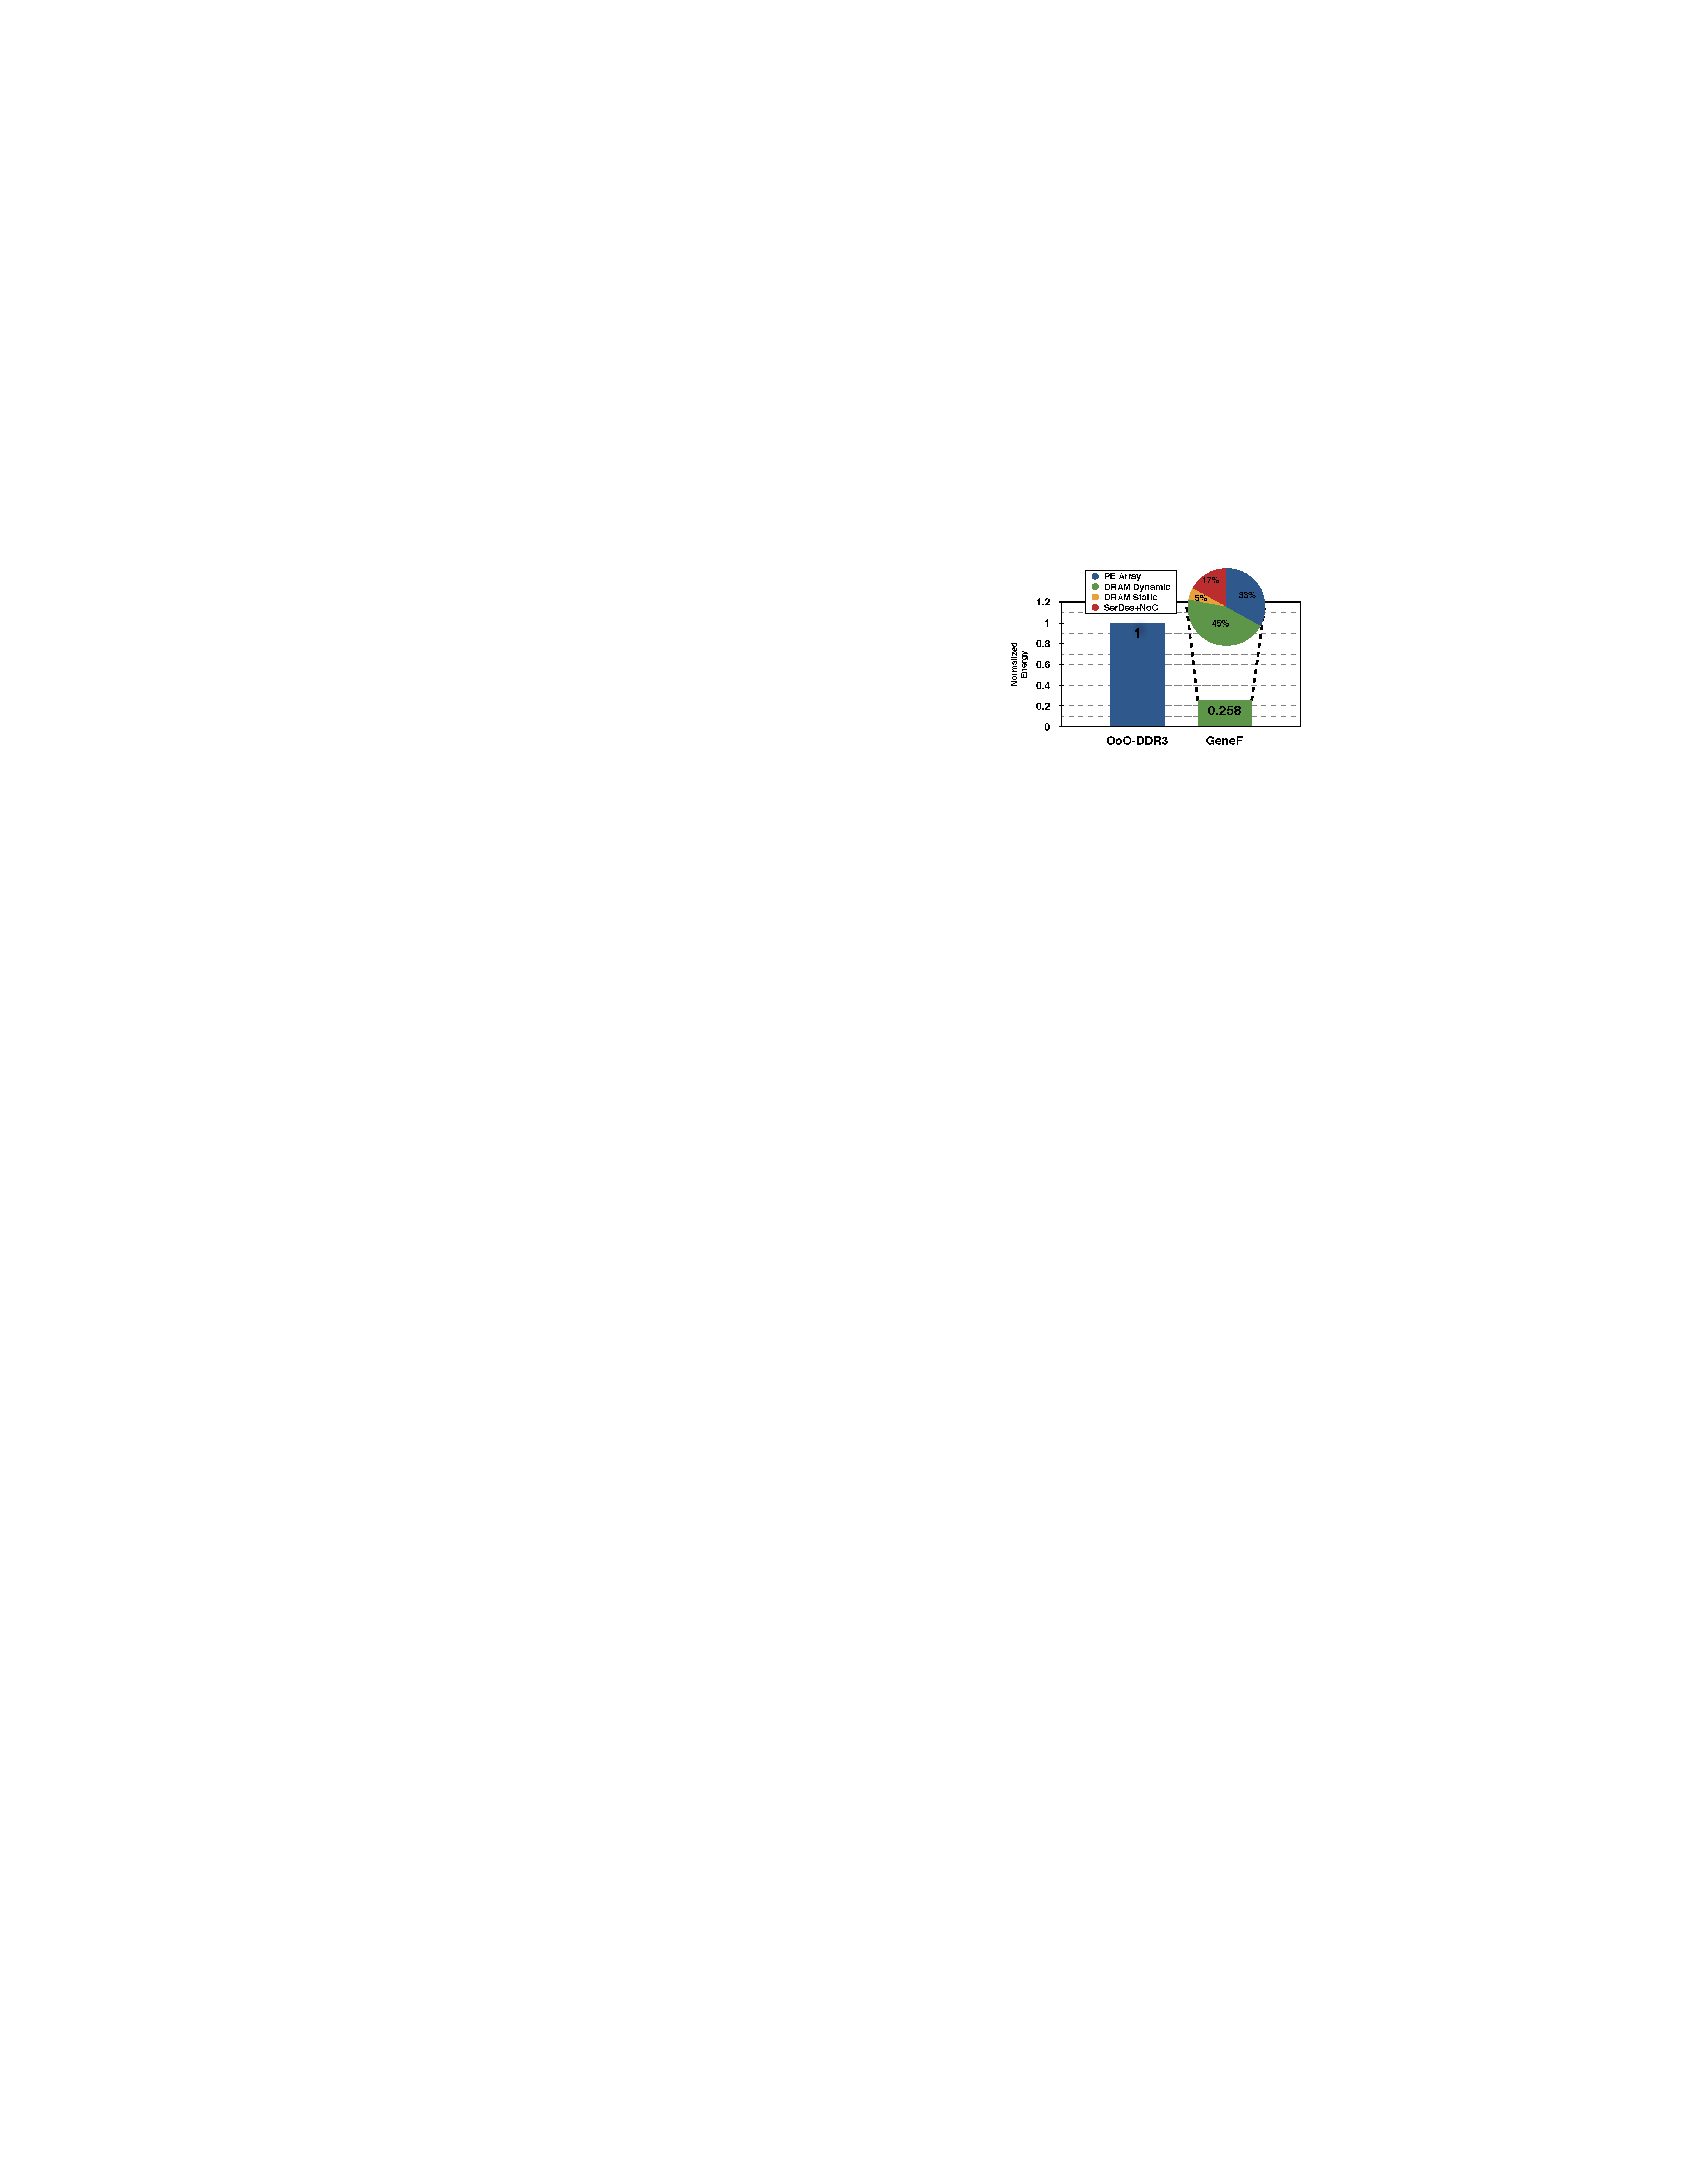
\includegraphics[scale=0.4]{fig/energy.pdf}
%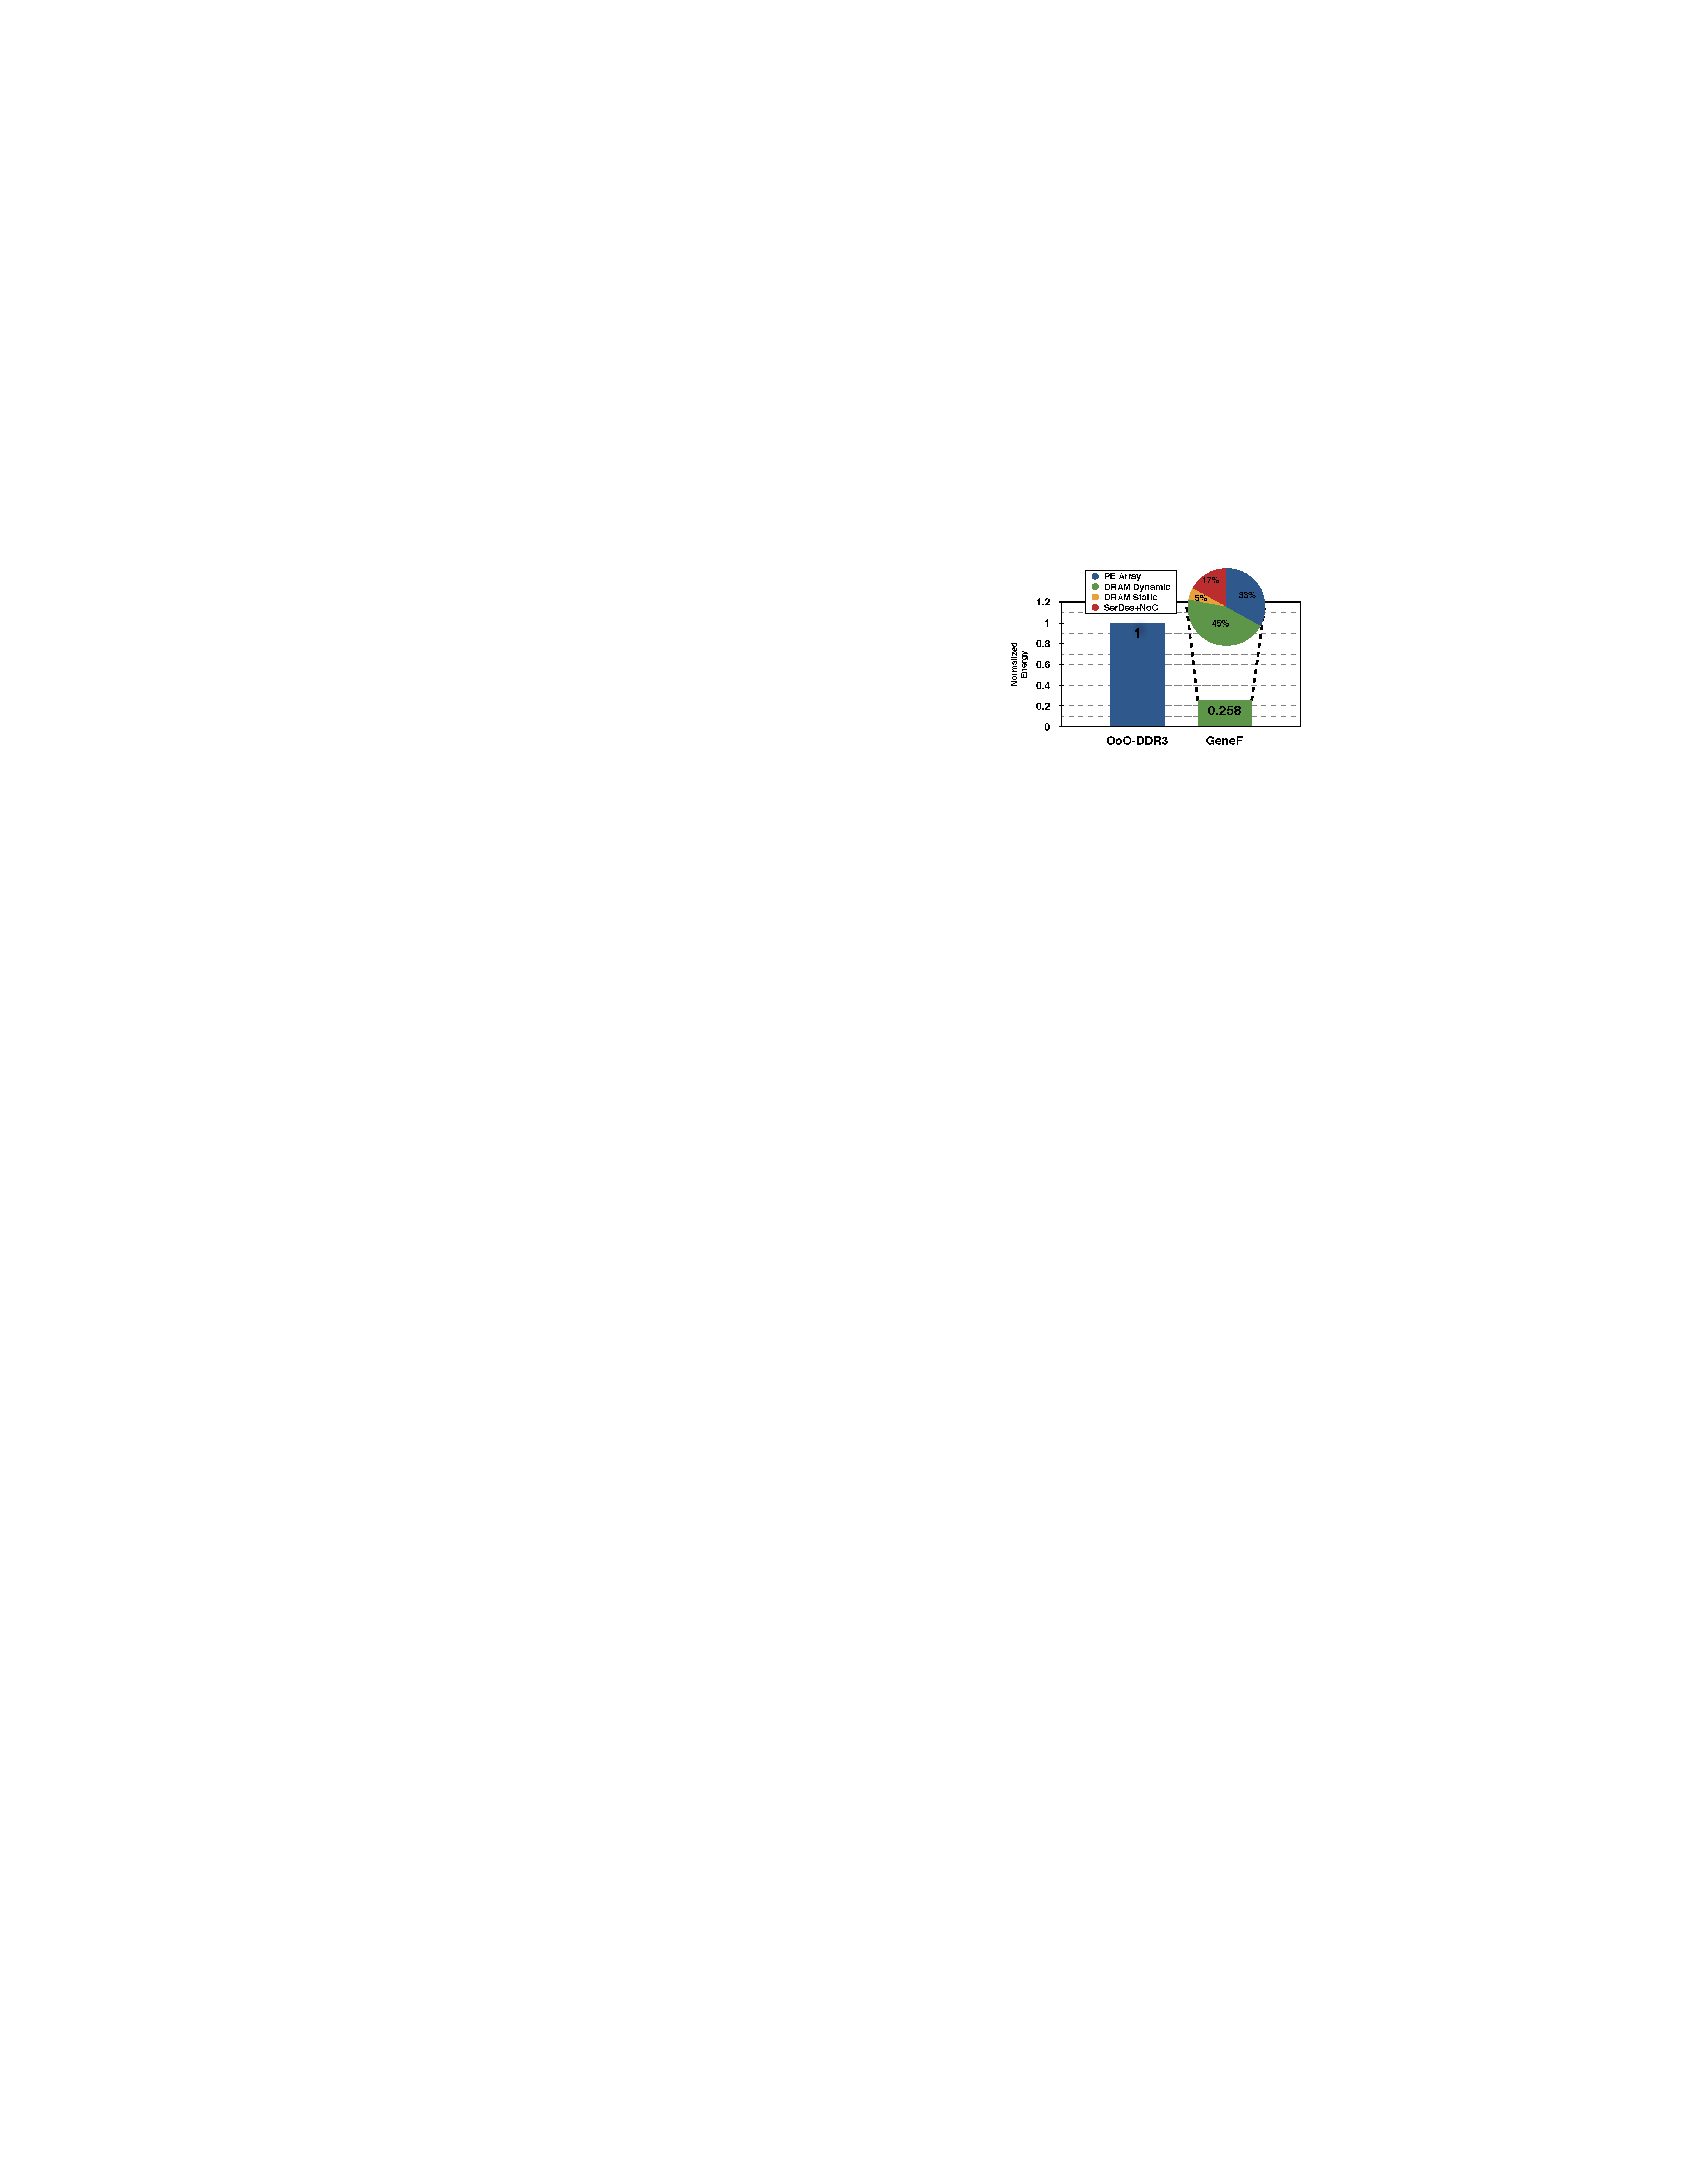
\includegraphics[width=\linewidth]{fig/energy.pdf}
\caption{GeneP area and power consumption}
\label{fig:energy}
\end{figure}

We found that the logic layer energy density of the accelerator is 20.7mW/mm$^{2}$ which is far below its upper limit of 133mW/mm$^{2}$. The area of PE logic of the accelerator is about 5.1mm2, which is only about 2.3\% of the entire logical layer area. We conclude that GeneF is thermally feasible and leads to greatly reduced energy consumption. GeneF achieved 7032$\times$ and 6687$\times$ energy efficiency in \textit{count stage} and \textit{determine stage}, respectively.

\section{Conclusion}
In this paper, we analyze compute and memory characteristics of FM-index, and find that data movement contributes to a significant portion of the total energy consumption. Our analysis reveals that the majority of this data movement comes from a number of simple functions. We revisit the processing-in-memory concept in the new context of (1) simple but effective integration of logic and memory through 3D stacking and (2) emerging genomic processing requires large amount of memory bandwidth. To this end, we propose a PIM accelerator for DNA alignment. GeneF fratures (1) many customized RISC-V based PEs inside a 3D stacking memory, (2) a light message mechanism that can hide remote access latency using in-place computing, (3) specialized prefetchers for simpler PE design. We showed that GeneF significantly outperforms traditional CPUs and ASIC implementations in terms of both performance and energy efficiency. We conclude that reducing data movement via processing-in-memory is a promising approach to improve both the performance and energy efficiency of genomic workloads in the future.

%%%%%%%%% -- BIB STYLE AND FILE -- %%%%%%%%
\bibliographystyle{ieeetr}
\bibliography{ref}

\end{document}
